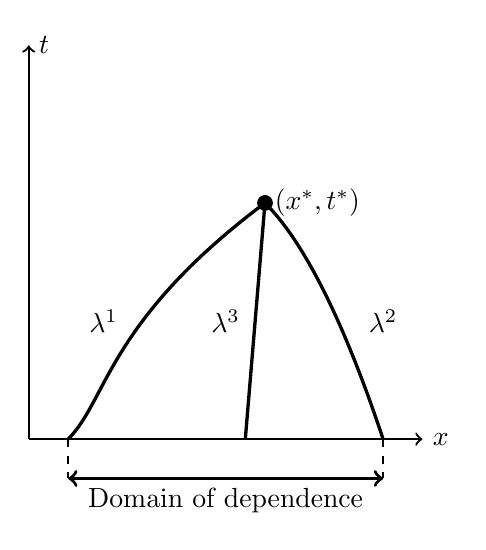
\begin{tikzpicture}
  \draw[thick,->](0,0)--(5,0) node [right] {$x$};
  \draw[thick,->](0,0)--(0,5) node [right] {$t$};
  \fill[black] (3,3) circle (0.1) node [right] {$(x^*,t^*)$};
  \draw[very thick] (0.5,0) .. controls (1.,0.5)and (1,1.5) .. (3.,3);
  \draw[very thick] (4.5,0) .. controls (4.,1.5) and (3.5,2.5) .. (3.,3);
  \draw[very thick] (2.75,0) -- (3.,3);
  \node at (0.95,1.5) {$\lambda^1$};
  \node at (2.5,1.5) {$\lambda^3$};
  \node at (4.5,1.5) {$\lambda^2$};
  \node[below] at (2.50,-0.5) {\text{Domain of dependence}};
  \draw[<->,very thick] (0.5,-0.5) -- (4.5,-0.5) ;
  \draw[dashed,thick] (0.5,0) -- (0.5,-0.5);
  \draw[dashed,thick] (4.5,-0.) -- (4.5,-0.5);
\end{tikzpicture}
%%% Local Variables:
%%% mode: latex
%%% TeX-master: "../../mainManuscript"
%%% End:
